\subsection{Development Board and Firmware}
In order to prototype our sensor node software, LoRaWAN gateway, and server, we are using
a development board that uses the same microcontroller and LoRa module that we are going to use for
our final design. That development board is the Seeed LoRa-E5 mini. The development board itself is
fairly barebones, containing only the LoRa module itself (the STM32WLE5JC), some I/O pins, a USB
Type-C input for power, and some antenna connectors. The board does not contain a USB-based
programmer, only SWD pins. Instead we had to purchase an external STLink programmer to be able to
connect the development board to our computer for programming. An image of the development board can
found in Figure \ref{fig:dev-board}.

\begin{figure}
    \centering
    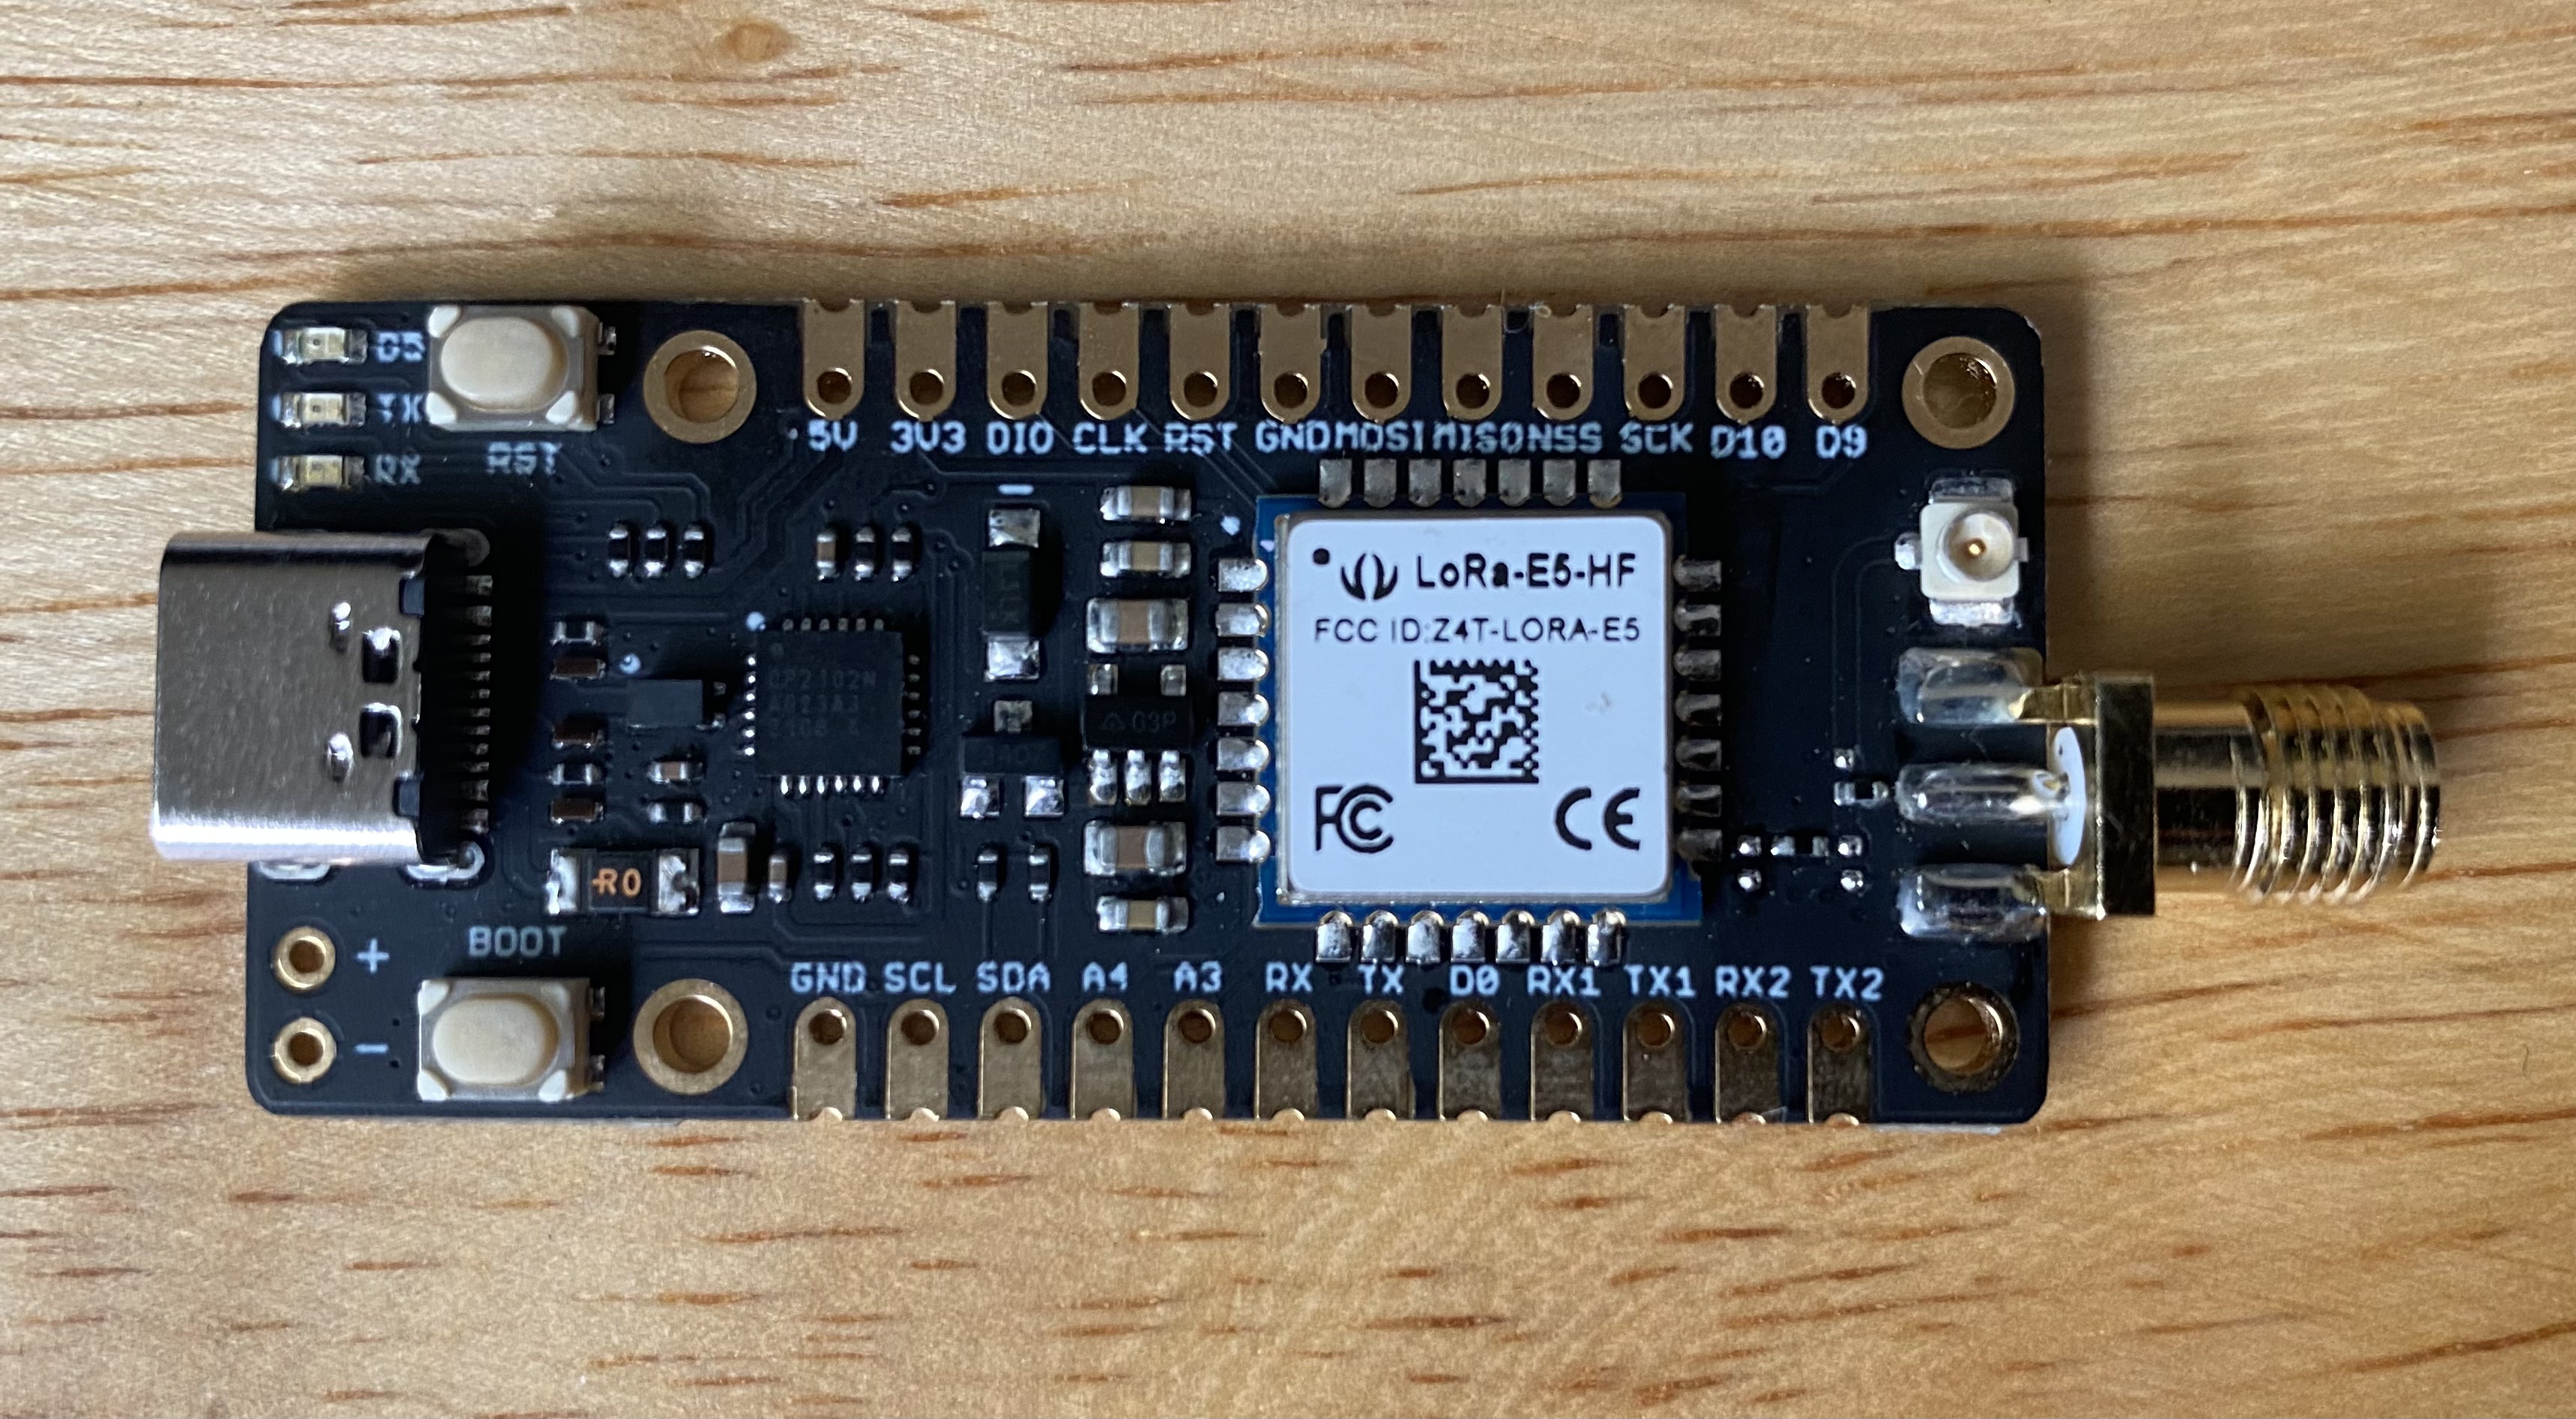
\includegraphics[width=4in]{figures/dev-board.png}
    \caption{The LoRa-E5 mini development board that we are using to prototype our software}
    \label{fig:dev-board}
\end{figure}

The initial prototype of the firmware will be done on the development board in tandem with a light
sensor (not used in the Aether node) to test taking readings of a sensor, and sending them over
LoRaWAN to the AWS LNS. The firmware developed in this stage might begin using a "barebones"
software architecture to become familiar with the MCU, but will eventually be converted to use
FreeRTOS. The prototype firmware will explore abstracting away the sensor details away to make it
easier to add new sensors later on and to decouple development of various sensors. This will allow
different sensors to more easily be developed simultaneously and not break existing code. Basic
loggings will be implemented over serial, but the CLI interface will not be developed at this stage
unless the project is ahead of schedule. 
